\documentclass[xcolor=dvipsnames]{beamer}
\mode<presentation> {

\usecolortheme{default}
%\setbeamercovered{transparent}

\definecolor{carolina}{HTML}{82CAFA}
%\definecolor{carolina}{HTML}{3BB9FF}
%\definecolor{gray}{HTML}{B6B6B4}
%\definecolor{dark}{HTML}{151B54}

\usetheme{Madrid}
\setbeamercolor{structure}{fg=carolina}
\setbeamercolor{block title}{bg=carolina}
\setbeamercolor{block title example}{bg=carolina}

%Uncomment the following if you prefer for the font color on carolina blue background to be black.
%\setbeamercolor{block title}{fg=black,bg=carolina}
%\setbeamercolor{frametitle}{fg=black}
%\setbeamercolor{title}{fg=black}

\setbeamertemplate{caption}[numbered]
\setbeamertemplate{enumerate items}[circle]
\setbeamertemplate{itemize items}[circle]
\setbeamertemplate{section in toc}[circle]
\setcounter{tocdepth}{1} 
\setbeamercolor{section in toc}{fg=black}

\usefonttheme[onlymath]{serif}

%\setbeamertemplate{footline} % To remove the footer line in all slides uncomment this line
%\setbeamertemplate{footline}[page number] 

% To replace the footer line in all slides with a simple slide count uncomment this line
%\setbeamertemplate{navigation symbols}{}

% To remove the navigation symbols from the bottom of all slides uncomment this line
}

%some commonly used packages
\usepackage{float}
\usepackage{graphics}
\usepackage{graphicx}
\usepackage{tikz}
\usepackage{fancyvrb}
\usepackage{comment}
\usepackage{amsmath}
\usepackage{amssymb}
\usepackage{lipsum}
\usepackage{subcaption}
\usepackage{caption}
\usepackage{comment}
\usepackage{multi row}
\usepackage{copyrightbox}
\usepackage{pdflscape}
\usepackage{url}
\usepackage{hyperref}

\newcommand{\overbar}[1]{\mkern 1.5mu\overline{\mkern-1.5mu#1\mkern-1.5mu}\mkern 1.5mu} %Instead of \bar or \overline, use \overbar for proper length and thickness bar for sample average. 

%Edit the following lump of code to customize with your name, title, and date
\title[R Markdown]{Presenting Your Analyses with R Markdown}
\author[Kevin Donovan]{Kevin Donovan}
\institute[UNC and IBIS]{UNC-Chapel Hill and IBIS Network}
\date[12/10/2020]{12/10/2020}

\newcounter{saveenumi}
\newcommand{\seti}{\setcounter{saveenumi}{\value{enumi}}}
\newcommand{\conti}{\setcounter{enumi}{\value{saveenumi}}}

\resetcounteronoverlays{saveenumi}

\begin{document}

\begin{frame}
	\titlepage
\end{frame}

\section{Presenting Your Results}
\begin{frame}
\frametitle{\insertsectionhead}
\begin{figure}
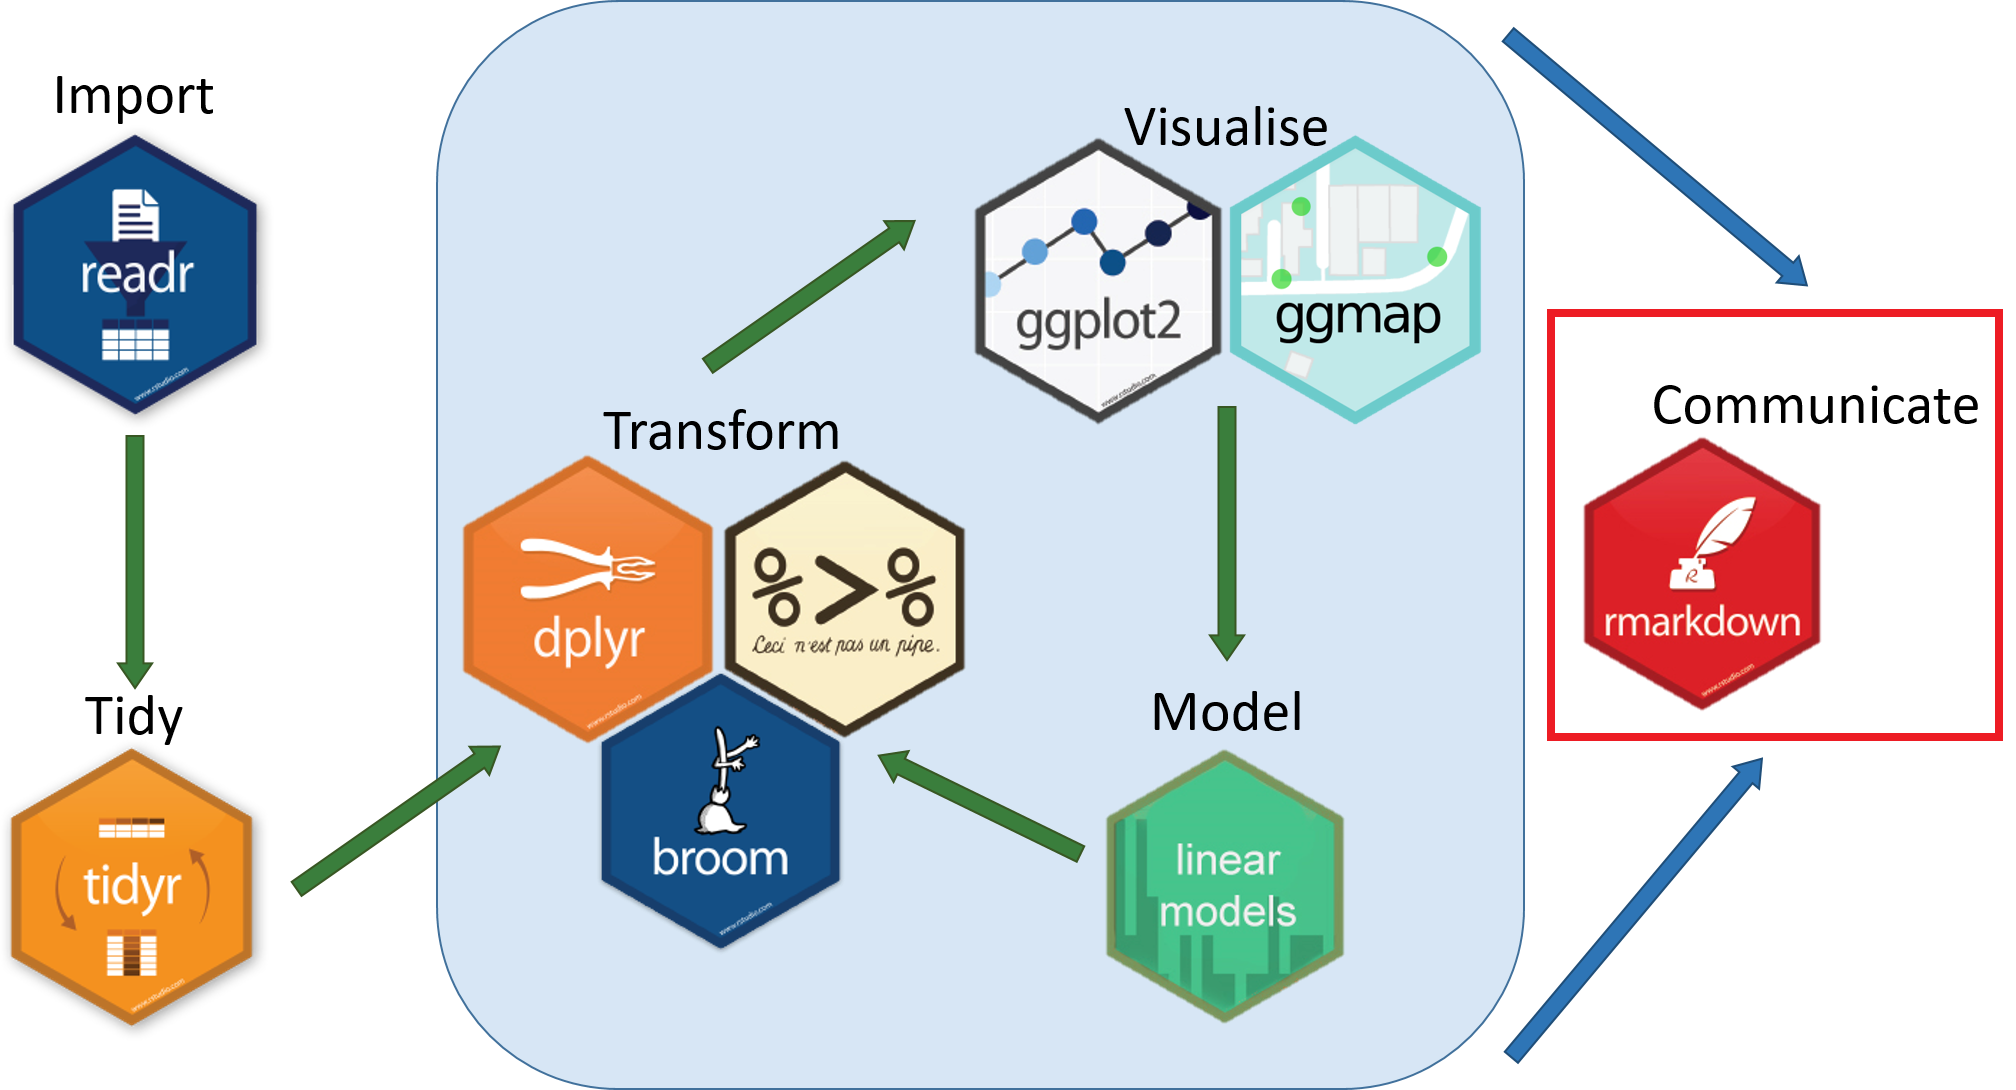
\includegraphics[scale=0.2]{images/tidyverse.png}
\end{figure}
\end{frame}

\begin{frame}
\frametitle{\insertsectionhead}
\textbf{Analysis contains:}
\begin{itemize}
\item Code
\item Tables
\item Plots
\item Notes
\end{itemize}
\textbf{Everything in separate files}
\begin{figure}
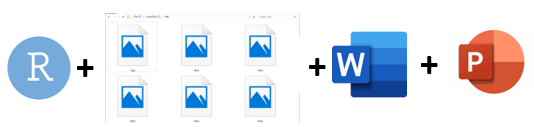
\includegraphics[scale=0.6]{images/logos_combined.png}
\end{figure}
\end{frame}

\begin{frame}
\frametitle{\insertsectionhead}
\textbf{R Markdown}\\
Single file containing all pieces
\begin{figure}
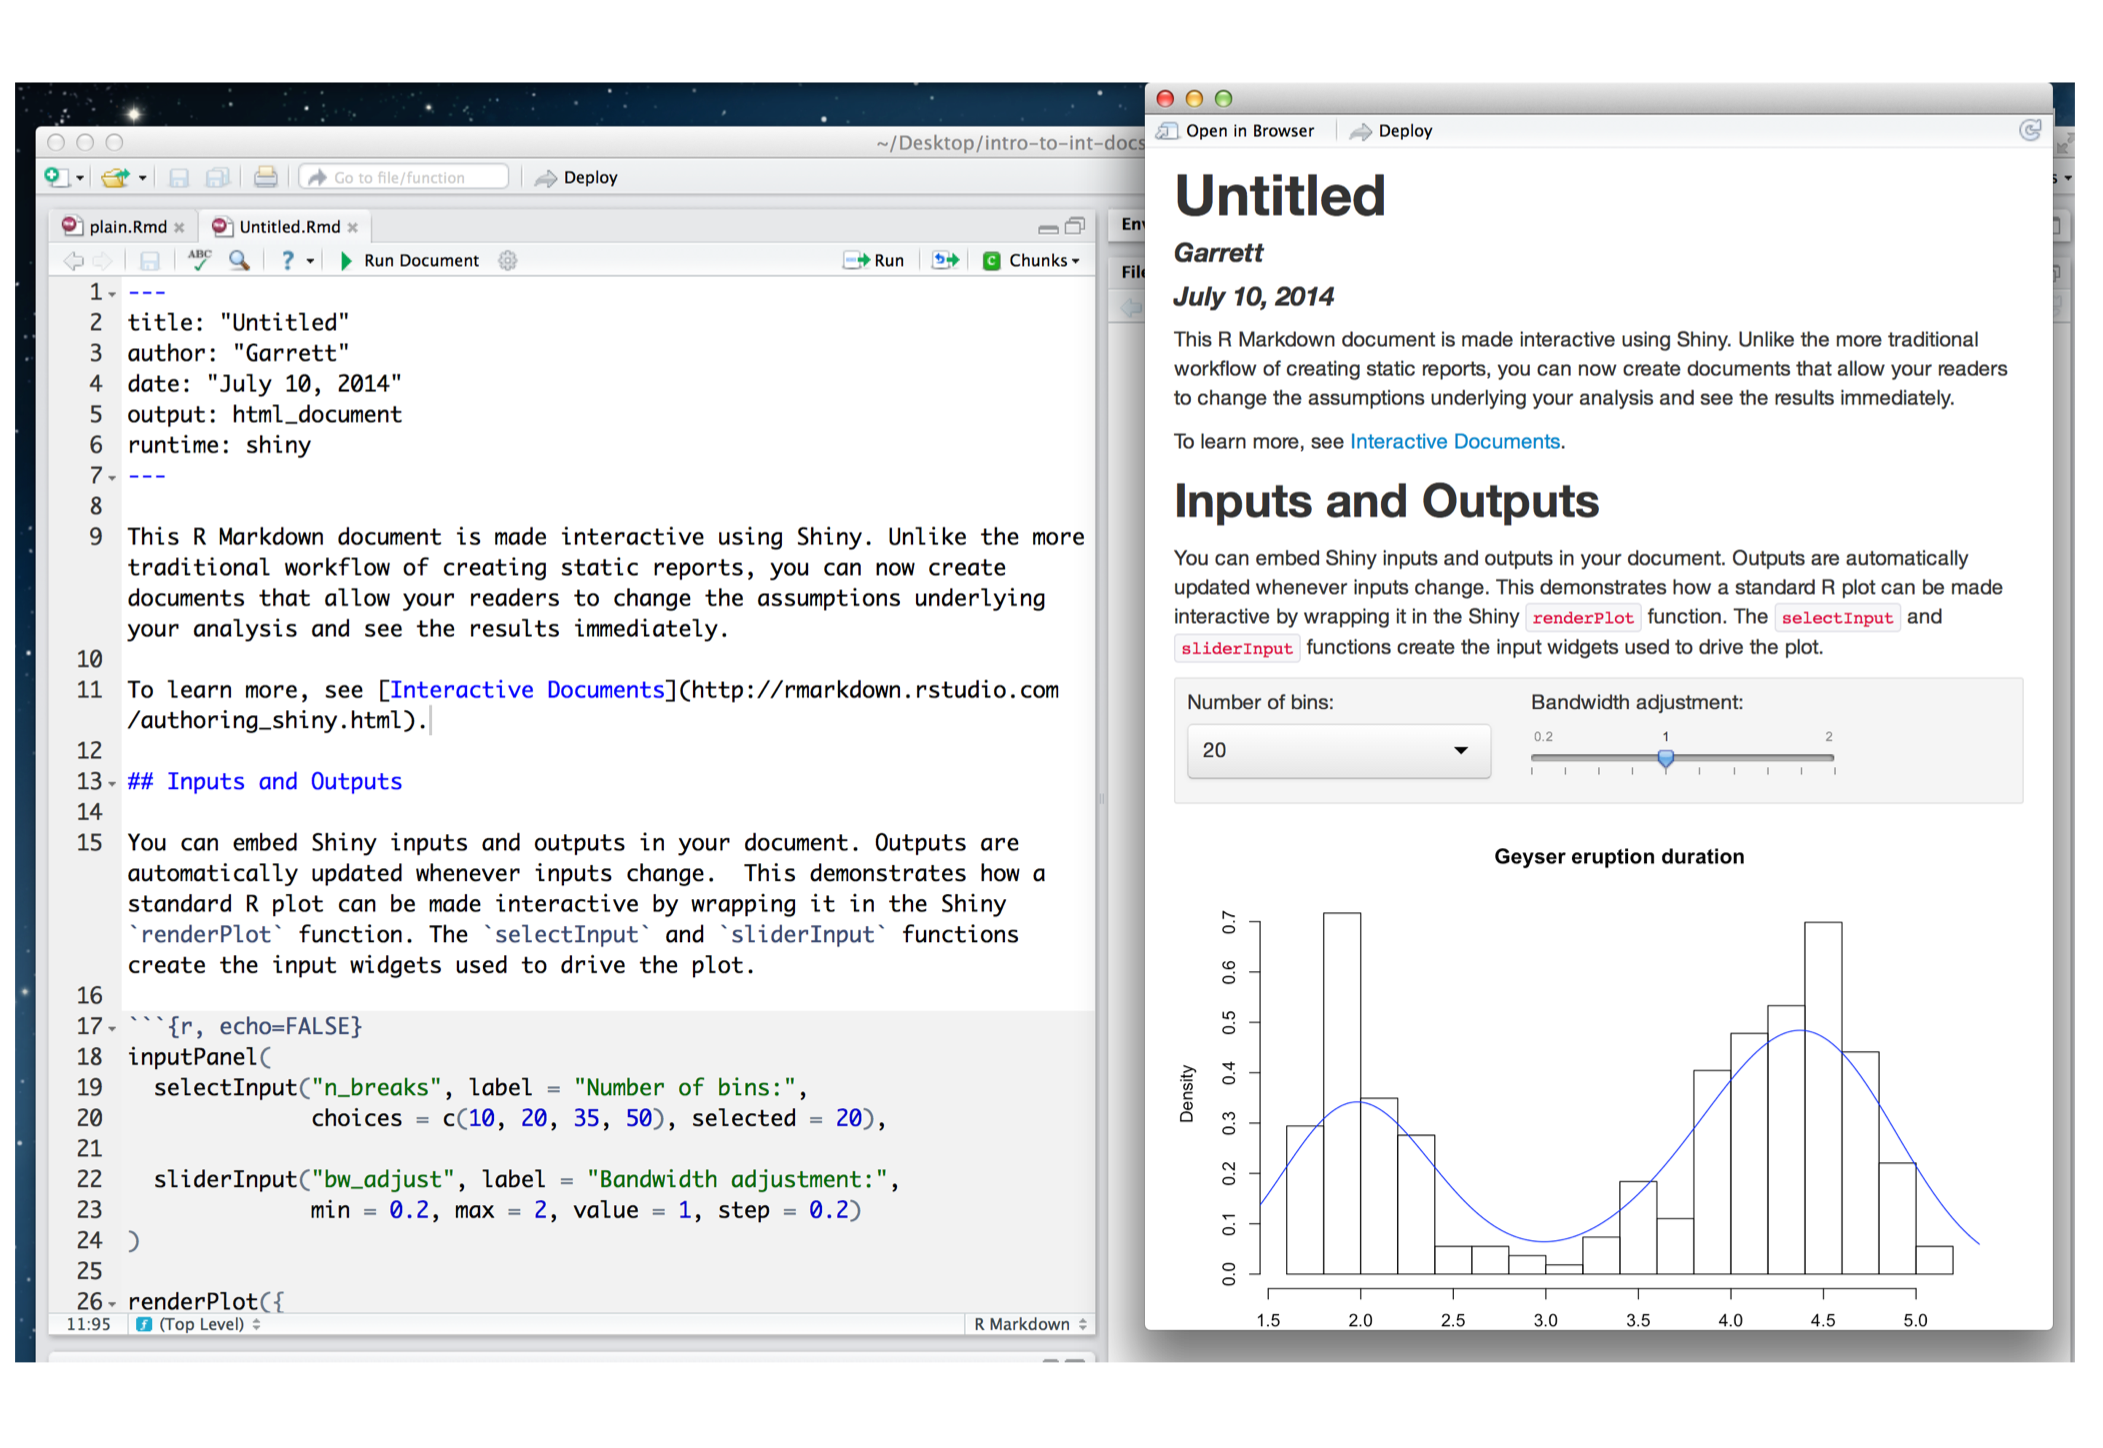
\includegraphics[scale=0.14]{images/rmd_intro.png}
\end{figure}
\end{frame}

\begin{frame}
\frametitle{\insertsectionhead}
Can compile output file into many different formats
\begin{figure}
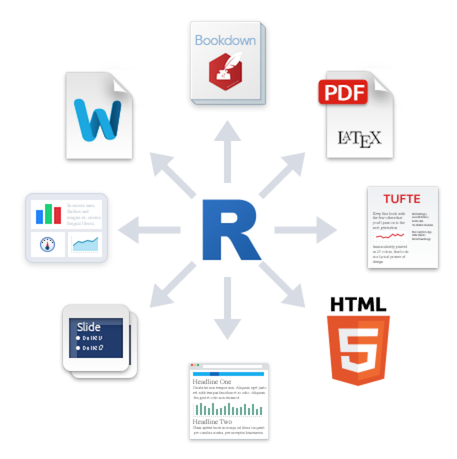
\includegraphics[scale=0.75]{images/rmd_formats.png}
\end{figure}
\end{frame}

\begin{frame}
\frametitle{\insertsectionhead}
Can compile output file into many different formats
\begin{figure}
	\centering
	\begin{subfigure}[t!]{0.49\textwidth}
	\centering
		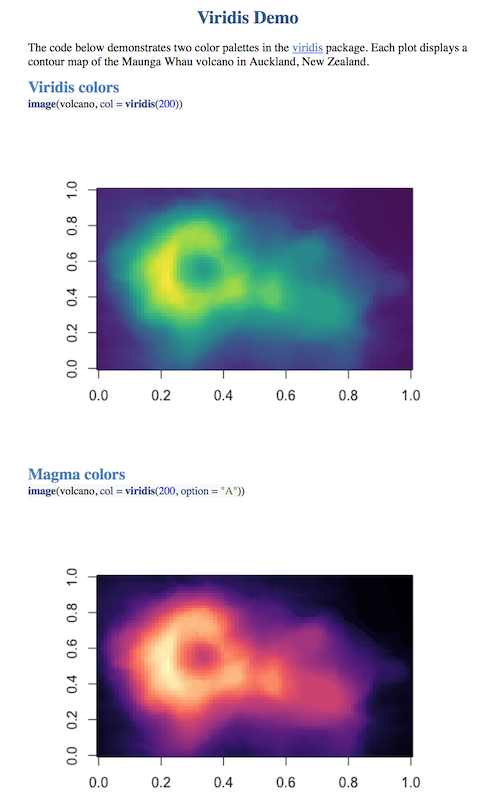
\includegraphics[width=0.75\linewidth]{images/rmd_doc.png}
	\end{subfigure}%
	\hfill
	\begin{subfigure}[t!]{0.49\textwidth}
	\centering
		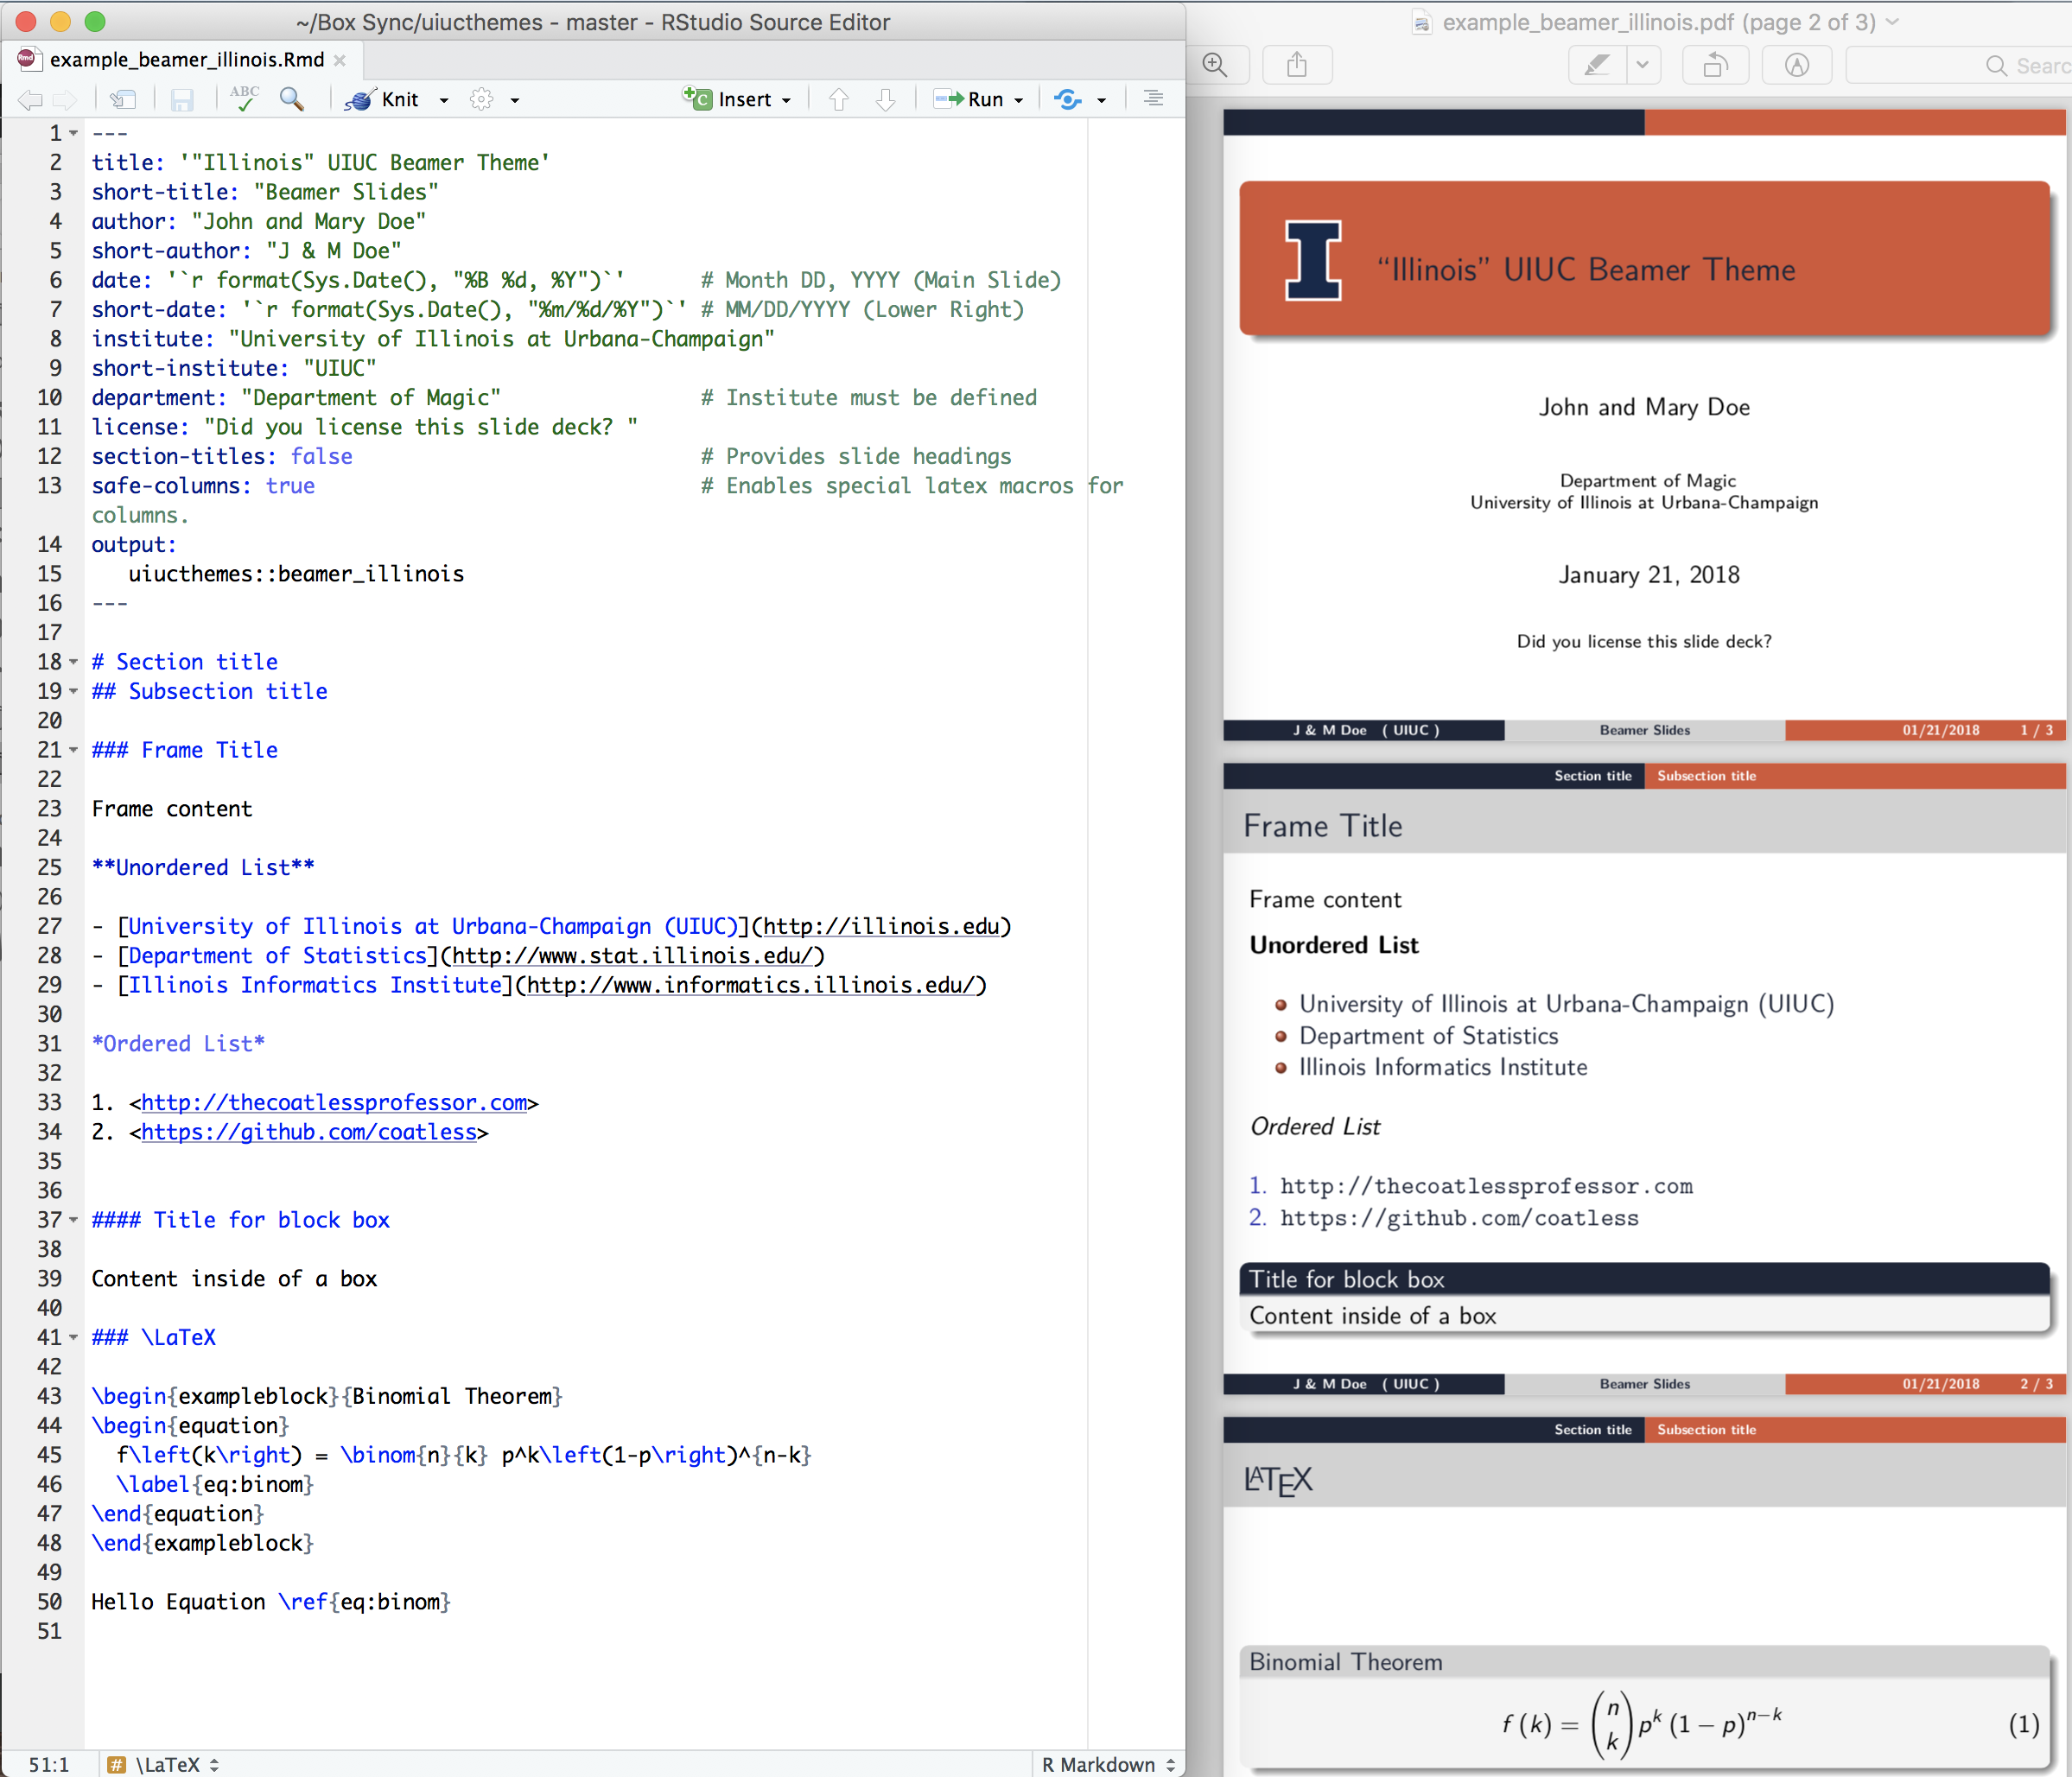
\includegraphics[width=1\linewidth]{images/rmd_slides.png}
	\end{subfigure}
\end{figure}
\end{frame}

\section{RMD File}
\begin{frame}
\frametitle{\insertsectionhead}
R Markdown defined by "enhanced" script = \textbf{.RMD file}
\begin{figure}
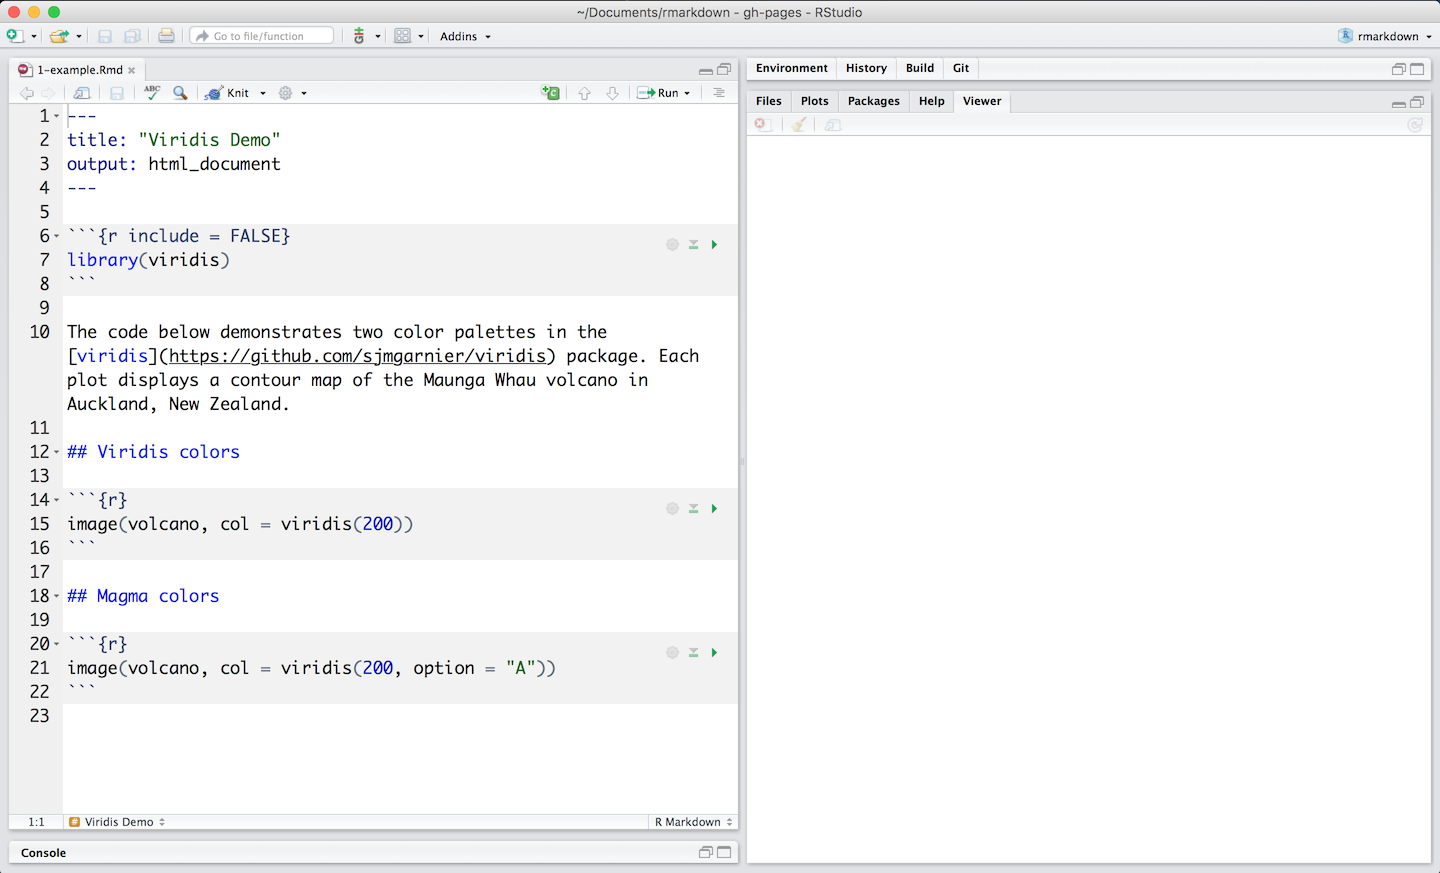
\includegraphics[scale=0.4]{images/rmd_file_example.png}
\end{figure}
\end{frame}

\section{RMD File}
\begin{frame}
\frametitle{\insertsectionhead}
\textbf{Script Structure}
\begin{figure}
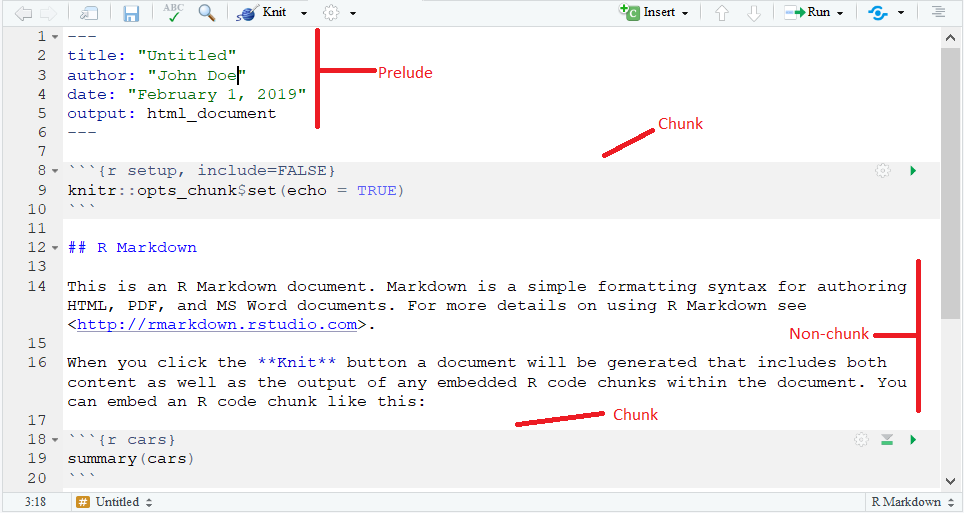
\includegraphics[scale=0.58]{images/Markdown_Ex.png}
\end{figure}
\end{frame}

\section{Kable with Markdown}
\begin{frame}
\frametitle{\insertsectionhead}
\color{blue}{
\textbf{\href{https://rfortherestofus.com/2019/11/how-to-make-beautiful-tables-in-r/}{Publication Quality Tables}}}
\begin{figure}
	\centering
	\begin{subfigure}[t!]{0.49\textwidth}
	\centering
		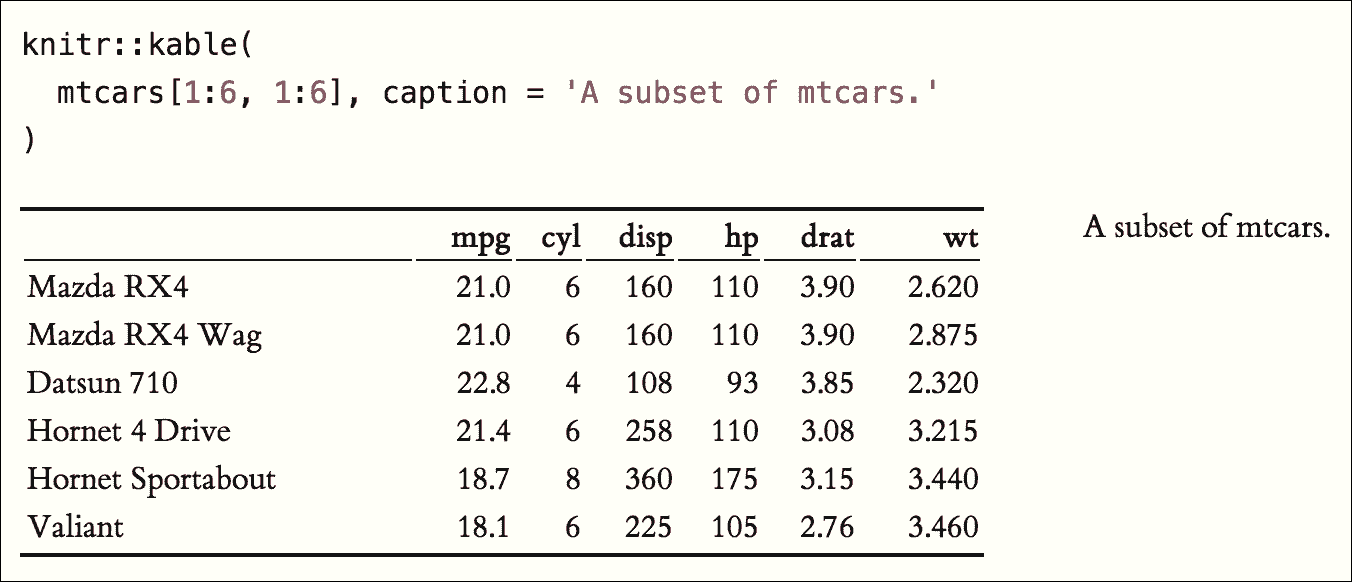
\includegraphics[width=1\linewidth]{images/kable_ex.png}
	\end{subfigure}%
	\hfill
	\begin{subfigure}[t!]{0.49\textwidth}
	\centering
		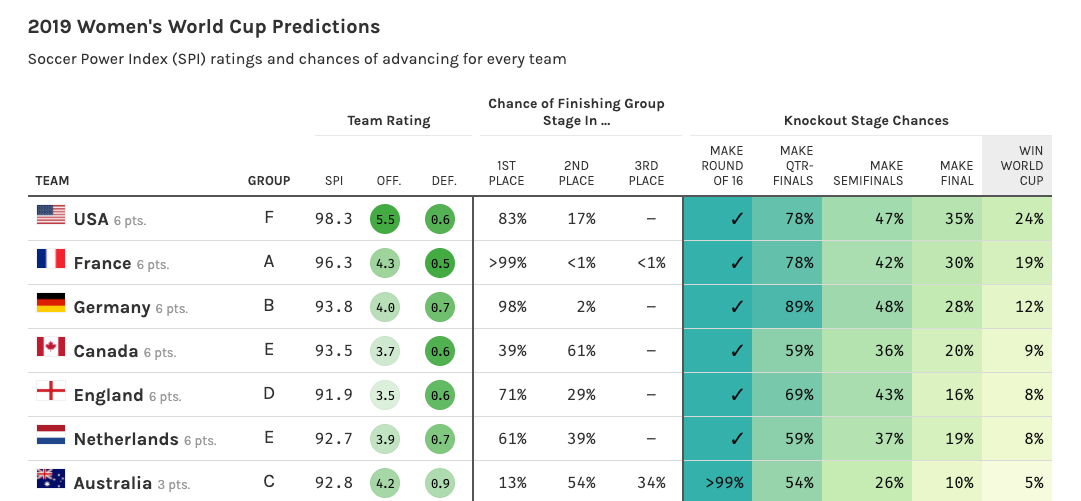
\includegraphics[width=1\linewidth]{images/table_nice.png}
	\end{subfigure}%
	\hfill
	\begin{subfigure}[t!]{0.49\textwidth}
	\centering
		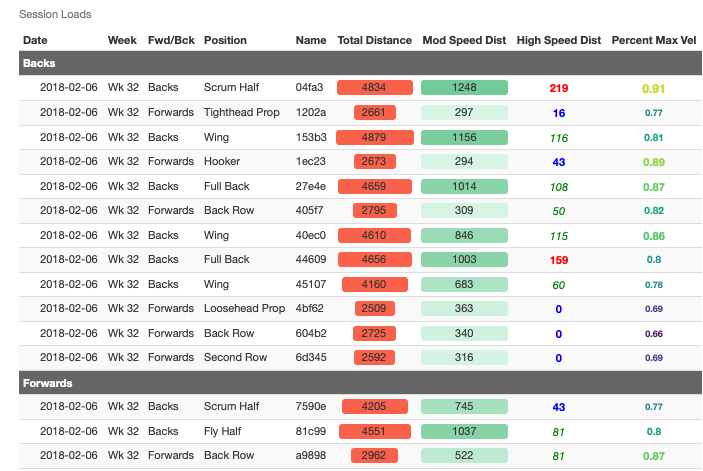
\includegraphics[width=1\linewidth]{images/table_nice_2.png}
	\end{subfigure}
\end{figure}
\end{frame}

\section{Song of the Session}
\begin{frame}
\frametitle{\insertsectionhead}
\href{https://www.youtube.com/watch?v=1qnV55LUFVM}{Bad Boy by BIGBANG}\\
\href{https://www.youtube.com/watch?v=2GRP1rkE4O0}{Blue by BIGBANG}
\begin{figure}

\includegraphics[scale=0.25]{images/song.jpg}
\end{figure}
\end{frame}

\end{document}

